%% Copernicus Publications Manuscript Preparation Template for LaTeX Submissions
%% ---------------------------------
%% This template should be used for copernicus.cls
%% The class file and some style files are bundled in the Copernicus Latex Package, which can be downloaded from the different journal webpages.
%% For further assistance please contact Copernicus Publications at: production@copernicus.org
%% https://publications.copernicus.org/for_authors/manuscript_preparation.html


%% Please use the following documentclass and journal abbreviations for preprints and final revised papers.

%% 2-column papers and preprints
\documentclass[esd, article]{copernicus}
\usepackage{booktabs}


%% Journal abbreviations (please use the same for preprints and final revised papers)


% Advances in Geosciences (adgeo)
% Advances in Radio Science (ars)
% Advances in Science and Research (asr)
% Advances in Statistical Climatology, Meteorology and Oceanography (ascmo)
% Annales Geophysicae (angeo)
% Archives Animal Breeding (aab)
% ASTRA Proceedings (ap)
% Atmospheric Chemistry and Physics (acp)
% Atmospheric Measurement Techniques (amt)
% Biogeosciences (bg)
% Climate of the Past (cp)
% DEUQUA Special Publications (deuquasp)
% Drinking Water Engineering and Science (dwes)
% Earth Surface Dynamics (esurf)
% Earth System Dynamics (esd)
% Earth System Science Data (essd)
% E&G Quaternary Science Journal (egqsj)
% European Journal of Mineralogy (ejm)
% Fossil Record (fr)
% Geochronology (gchron)
% Geographica Helvetica (gh)
% Geoscience Communication (gc)
% Geoscientific Instrumentation, Methods and Data Systems (gi)
% Geoscientific Model Development (gmd)
% History of Geo- and Space Sciences (hgss)
% Hydrology and Earth System Sciences (hess)
% Journal of Bone and Joint Infection (jbji)
% Journal of Micropalaeontology (jm)
% Journal of Sensors and Sensor Systems (jsss)
% Magnetic Resonance (mr)
% Mechanical Sciences (ms)
% Natural Hazards and Earth System Sciences (nhess)
% Nonlinear Processes in Geophysics (npg)
% Ocean Science (os)
% Polarforschung - Journal of the German Society for Polar Research (polf)
% Primate Biology (pb)
% Proceedings of the International Association of Hydrological Sciences (piahs)
% Scientific Drilling (sd)
% SOIL (soil)
% Solid Earth (se)
% The Cryosphere (tc)
% Weather and Climate Dynamics (wcd)
% Web Ecology (we)
% Wind Energy Science (wes)


%% \usepackage commands included in the copernicus.cls:
%\usepackage[german, english]{babel}
%\usepackage{tabularx}
%\usepackage{cancel}
%\usepackage{multirow}
%\usepackage{supertabular}
%\usepackage{algorithmic}
%\usepackage{algorithm}
%\usepackage{amsthm}
%\usepackage{float}
%\usepackage{subfig}
%\usepackage{rotating}


\begin{document}

\title{Potential for bias in effective climate sensitivity from state-dependent energetic balance}


% \Author[affil]{given_name}{surname}

\Author[1]{Benjamin M.}{Sanderson}
\Author[2]{Maria}{Rugenstein}


\affil[1]{CERFACS, Toulouse, France}
\affil[2]{Colorado State University, Fort Collins CO, USA}



\correspondence{Benjamin Sanderson (sanderson@cerfacs.fr)}

\runningtitle{state-dependent energetic balance}

\runningauthor{Sanderson et al.}





\received{}
\pubdiscuss{} %% only important for two-stage journals
\revised{}
\accepted{}
\published{}

%% These dates will be inserted by Copernicus Publications during the typesetting process.


\firstpage{1}

\maketitle



\begin{abstract}
Effective climate sensitivity is the standard approach for calculating the equilibrium response of the a climate model to a change in greenhouse gas forcing.  Temperatures are linearly extrapolated as a function of top of atmosphere energetic imbalance to estimate the temperature change in an equilibrated state (given full equilibration occurs on timescales of millennia).   In this study, we consider an alternative approach for estimating equilibrium climate sensitivity through Bayesian calibration of a multiple timescale simple climate model.  Though the method leaves large uncertainties in ECS using conventional 150 year CO2 quadrupling experiments, application to millennial timescale experiments in LongrunMIP allows for robust fitting of long term tendencies, allowing for a partially independent assessment of effective climate sensitivity estimates.  Results suggest potential biases in effective sensitivity estimates in the case of particular models where persistent radiative imbalances are present, given that imbalances are shown to differ between pre-industrial and quadrupled CO2 states.  These biases may imply a reconsideration of certain model published values of climate sensitivity, and the presence of radiative imbalances in a number of CMIP5 and CMIP6 models underlines the urgent requirement for operational climate sensitivity experiments on millennial timescales to assess if such biases exist in existing model estimates of climate sensitivity in the wider CMIP ensembles. 
\end{abstract}


%\copyrightstatement{TEXT} %% This section is optional and can be used for copyright transfers.


\introduction  
Equilibrium Climate Sensitivity (ECS) of an Earth System Model is the equilibrium increase in global mean temperature experienced in response to an instantaneous doubling change in carbon dioxide concentrations.  Introduced as a metric of response of the Earth System to greenhouse gases in the early years of computational climate science \citep{charney1979carbon,hansen1984climate}, it remains a very common metric of the sensitivity of the Earth to greenhouse gas forcing \cite{knutti2017beyond,stocker2013climate}.

Measuring ECS in a coupled climate model, however, is difficult owing to the time required for the equilibration of the system to a change in forcing \cite{wetherald2001committed,solomon2010persistence,jarvis2011contribution}. necessitating simulations of multiple millennia to obtain a near-equilibrated estimate of temperature response \cite{rugenstein2020equilibrium}.  The computational burden of conducting such simulations implies that standard practise for model assessment \citep{stocker2013climate,forster2016inference,andrews2012forcing} is to measure an "Effective Climate Sensitivity" (EffCS) using feedbacks extrapolated from those measures in the first 150 years of a quadrupled CO$_2$ simulation \cite{gregory2004new,murphy1995transient}.

Recent work, however, has highlighted potential uncertainties in the EffCS approximation of ECS - studies have found that net radiative feedbacks can exhibit both timescale dependencies \cite{proistosescu2017slow,andrews2018accounting} and state dependencies \citep{pfister2017state,bloch2021climate} both of which draw into question the implicit constant feedback assumption used in the derivation of EffCS.

The LongrunMIP project set out in part to quantify this error by running a subset of Earth System Models in idealised carbon dioxide perturbation experiments with simulations of millennial timescale response \citep{rugenstein2019longrunmip}.  Initial studies compared the EffCS as derived using the first 150 years of the simulation with that derived using the last 15 percent of warming in multi-thousand year experiments - finding that the accuracy of the EffCS varied by model, but in most cases represented a 10$\%$ error or less in the estimate of ECS \cite{rugenstein2020equilibrium}.

A general assessment of the likely range of EffCS \citep{sherwood2020assessment} explicitly requires prior assumptions on the ratio of ECS:EffCS (represented by a parameter $\zeta$ such that ECS/EffCS is given by $(1+\zeta)$), given that the confidence in headline upper bound of EffCS in the study rests on combined evidence of paleo evidence and recent historical evidence.  The paleo evidence represents the near-equilibrium response, so prior confidence that $\zeta$ is small, itself arising from LongrunMIP \citep{rugenstein2020equilibrium}, contributes to the headline result that values of EffCS of greater than 4.5K are unlikely.

The findings of \cite{sherwood2020assessment} somewhat challenge the use of the CMIP6 ensemble of climate models \citep{eyring2016overview} as a proxy for climate projection uncertainty in assessment \citep{o2016scenario}, given approximately 1/3 of the ensemble \citep{meehl2020context} have EffCS values of greater than  4.7K (the 95th percentile of the distribution as assessed by \cite{sherwood2014spread}).  The high EffCS values in CMIP6 have been attributed to stronger positive cloud feedbacks \cite{zelinka2020causes}.  
So how plausible are the higher sensitivity models?  Studies have found that one of the higher sensitivity models (CESM2) tend to perform more poorly in paleoclimate simulations than its lower sensitivity predecessors \citep{zhu2020high}.  Although studies \citep{nijsse2020emergent,tokarska2020past} suggest that post-1980 warming may help constrain the Transient Climate Response (the warming expected at time of CO$_2$ doubling in an experiment with a 1 percent annual concentration increase), the constrain on EffCS from historical warming alone is weaker both in terms of correlations in the CMIP ensemble \cite{tokarska2018cumulative} and in ensembles of simple models \cite{sanderson2020relating,sherwood2020assessment}.

A core assumption in the calculation of EffCS is that the system will ultimately stabilise in a state of energetic balance \cite{gregory2004new}.  However, in practise a number of models exhibit energetic radiative top of atmosphere imbalances in the control state \cite{rugenstein2019longrunmip}, and as such the Effective Climate Sensitivity is calculated using net flux anomalies relative to the control mean top of atmosphere net radiative fluxes.  However, it remains untested as to whether such models will ultimately converge to the same state of imbalance.

In the present study, we consider an alternative approach for calculating climate sensitivity from a climate simulation in which there is a step change in carbon dioxide concentrations.  We consider how the method of calculating effective climate sensitivity, either from initial response or from millennial scale simulations, may be potentially subject to biases arising from assumptions on the equilibrated radiative state.  Finally, we consider how these uncertainties may relate to our confidence in the relationship between transient and equilibrium climate feedbacks.

\section{Methods}
\label{sec_methods}
We consider available pre-industrial control simulations (PICTRL) and abrupt CO2 quadrupling experiments (ABRUPT4X) from 3 available ensembles: CMIP5 \citep{taylor2012overview}, CMIP6 \citep{eyring2016overview} and LongRunMIP \cite{rugenstein2019longrunmip}.  From each of these, we compute global averages of surface temperature, plus top of atmosphere shortwave and longwave fluxes.

We assume that the temperature and radiative timeseries can be modelled by a sum of exponential decay terms, a basis set \cite{proistosescu2017slow,sanderson2020relating} which is consistent with the general solution of two layer simple climate models with \cite{geoffroy2013transient,winton2010importance,smith2018fair} or without \cite{geoffroy2013constant} terms for ocean heat uptake efficacy.  

As in \cite{proistosescu2017slow}, we allow for three independent equilibration timescales, such that:

\begin{subequations}
\begin{align}
   T(t)&=\sum_{n=1}^3 S_n(1-e^{-(t/\tau_n)})+T_0\label{eq1}\\
   R(t)&=\sum_{n=1}^3 R_n(1-e^{-(t/\tau_n)})+R^{4x}_{0}\label{eq2}\\
\end{align}
\end{subequations}

Where $T(t)$ and $R(t)$ are the global annual mean surface temperature and net top of atmosphere radiative flux timeseries respectively, $tau_n$ is the decay time associated with the timescale $n$, $S_n$ and $R_n$ are scaling factors and $T_0$ and $R_0$ are constant terms. $T_0$ is taken as the mean temperature in the last available 500 years of the control simulation.  $R^{4x}_0$ represents the radiative flux imbalance at $t=0$ and is calibrated during the analysis.  


\subsection{Bayesian Calibration of long term response parameters}
We fit the response equations detailed in \ref{eq1} to the output of each ensemble member's global mean radiative flux and surface temperature timeseries using a Markov Chain Monte Carlo optimizer \cite{foreman2013emcee} (as implemented in the 'lmfit' Python module), allowing for $n=3$ representative decay timescales.  Parameter ranges are constrained according to Table \ref{tb1}.  

\begin{table}[]
    \centering
    \begin{tabular}{l|l|l|c|c}
    Parameter & long name & Units & Min value & Max value \\
    $S_1$ & Short timescale sensitivity & K & 0 & 10 \\
    $S_2$ & Intermediate timescale sensitivity & K & 0 & 10 \\
    $S_3$ & Long timescale sensitivity & K & 0 & 10 \\
    $T_0$ & Control mean temperature & K & n/a & n/a \\
    $\tau_1$ & Short timescale & years & 0 & 10 \\
    $\tau_2$ & Intermediate timescale & years & 100 & 150 \\
    $\tau_3$ & Long timescale & years & 150 & 2000 \\
    $R_0$ & Equilibrium energy leak (PICTRL) & Wm$^{-2}$ & -5 & 5 \\
    \end{tabular}
    \caption{Parameters and prior ranges considered in the Bayesian calibration of equation \ref{eq1}.  $T_0$ is predefined as the mean temperature in the last 500 years of PICTRL. }
    \label{tb1}
\end{table}

The conventional effective climate sensitivity $S_{eff}$ is calculated using the first 150 years of simulation.   For the calculation of effective climate sensitivities, control global mean temperatures and TOA energetic imbalances are expressed as anomalies relative to $T_0$, estimated as the last 100 available years of the PICTRL simulation (if fewer than 500 PICTRL years are available, all available years are used).  A second estimate of long term equilibrium warming, $S_{LR}$, follows \cite{rugenstein2020equilibrium}, by calculating the effective climate sensitivity based on the years corresponding to the last 15$\%$ of warming in the simulation (that is, for all years following the point when the simulation first exceeds 85$\%$ of the average global mean temperature anomaly  in the last 20 years of the ABRUPT4X simulation).

We finally calculate a third estimate of climate sensitivity $S_{extrap}$ as in Eq. \ref{eq3} in the equilibrated abrupt4xCO2 simulation using the ensemble of fitted parameters from Bayesian calibration of Equation \ref{eq1}, using again global mean temperature anomalies from ABRUPT4X relative to $T_0$ (taken as mean temperatures over the last 100 years of PICTRL).  

\begin{align}
   T_{extrap}&=\sum_{n=1}^3 S_n+T_0
\label{eq3}
\end{align}

We estimate the long term radiative imbalance in the ABRUPT4X simulation from the fitted values for $R_0$ (the initial forcing at $t=0$ in ABRUPT4X) and $R_n$ (the amplitude of the decay in forcing at the timescale corresponding to $\tau_n$) from equation \ref{eq2}.

\begin{align}
   R^{4x}_{extrap} &=\sum_{n=1}^3 R_n+R^{4x}_0,
\label{eq4}
\end{align}

where $R^{4x}_{extrap}$ is the estimate of long term radiative imbalance in the ABRUPT4X simulation

$R^{CTRL}_0$, the radiative imbalance in the control simulation is assessed as the time average of net Top of Atmosphere (TOA) flux from the last 100 years of PICTRL.  In fully equilibrated models with no energetic leaks, it would be expected that $R^{CTRL}=0$, but it has been noted previously that this is not always the case and small energetic imbalances remain in some models even after the model global mean temperature trends have ceased \citep{rugenstein2019longrunmip}.



\subsection{Results}
The results for the fitted exponential models for ABRUPT4X simulations in the LongRunMIP archive are presented in Figure \ref{fig:greg_lrmip}.  We assess equilibrium estimates of warming and TOA energetic imbalance using the approach of \cite{rugenstein2020equilibrium} - where the last 15$\%$ of warming is used to estimate long term effective climate sensitivity  \citep{gregory2004new} subject to an assumption that the TOA imbalance in the control and 4xCO2 equilibrated state are identical.  This estimate is referred to as $S_{LR}$, and is compared with $S_{eff}$, the more commonly available estimate of effective climate sensitivity calculated with the first 150 years of data.

\begin{figure}
    \centering
    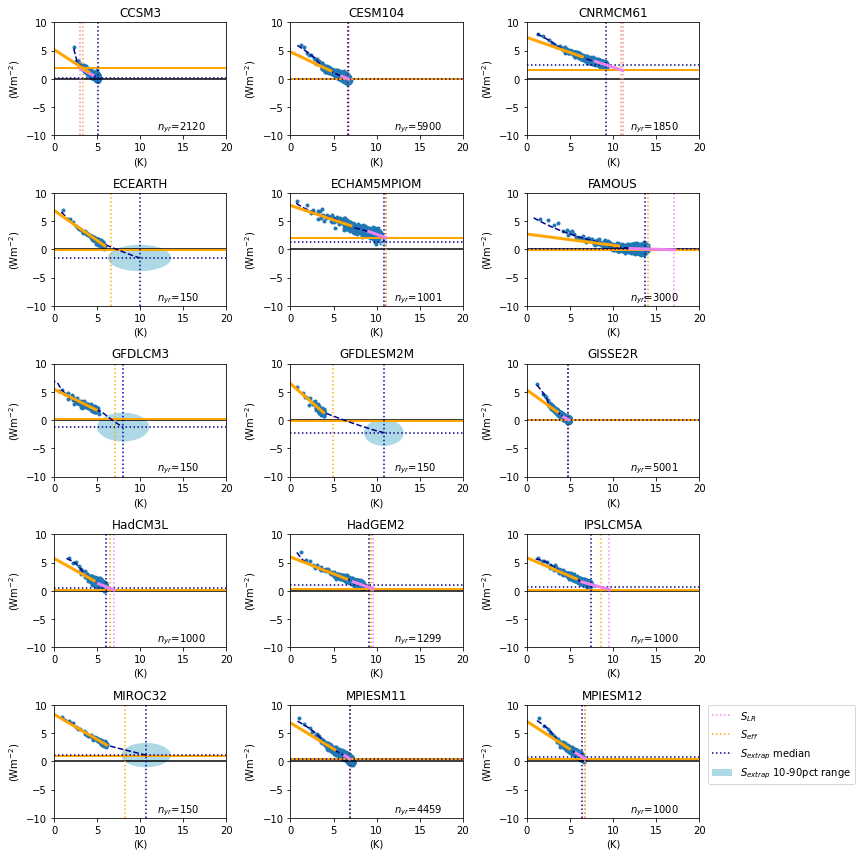
\includegraphics[width=\linewidth]{greg_lrmip.png}
    \caption{An illustration of global mean net radiative imbalance as a function of surface temperature for different members of the LongrunMIP archive.  Vertical axis shows absolute top of atmosphere net radiative imbalance, horizontal axis shows surface temperature relative to the final 500 years of the control simulation.  Blue points are individual years from ABRUPTP4X.  Yellow solid horizontal line show the PICTRL net energy imbalance averaged over the final 100 years of the simulation.   Solid yellow and pink lines show linear regressions used to estimate effective climate sensitivity using the first 150 years of data (yellow) and the last 15$\%$ of warming (pink), vertical dotted pink and yellow lines show corresponding values of effective climate sensitivity.  Dashed blue lines show the maximum likelihood exponential model fit using all available years in the simulation, while light blue ellipse shows the 5-95 confidence intervals for the corresponding values of $S_{extrap}$
     }
    \label{fig:greg_lrmip}
\end{figure}

We then compare the results with the approach detailed in Section \ref{sec_methods} , where the equilibrium warming $S_{extrap}$ (shown in Figure \ref{fig:t_extrap_lrmip}) and energetic imbalance $R^{4x}_{extrap}$ (shown in Figure \ref{fig:extrap_lrmip}) are estimated from the available data.  This estimate is subject to large errors in 150 year simulations (illustrated here by the 10th and 90th percentiles of the fitted range in the MCMC fitting process), but is relatively precise for the multi-millennial simulations in LongrunMIP (see Figure \ref{fig:t_extrap_lrmip})

\begin{figure}
    \centering
    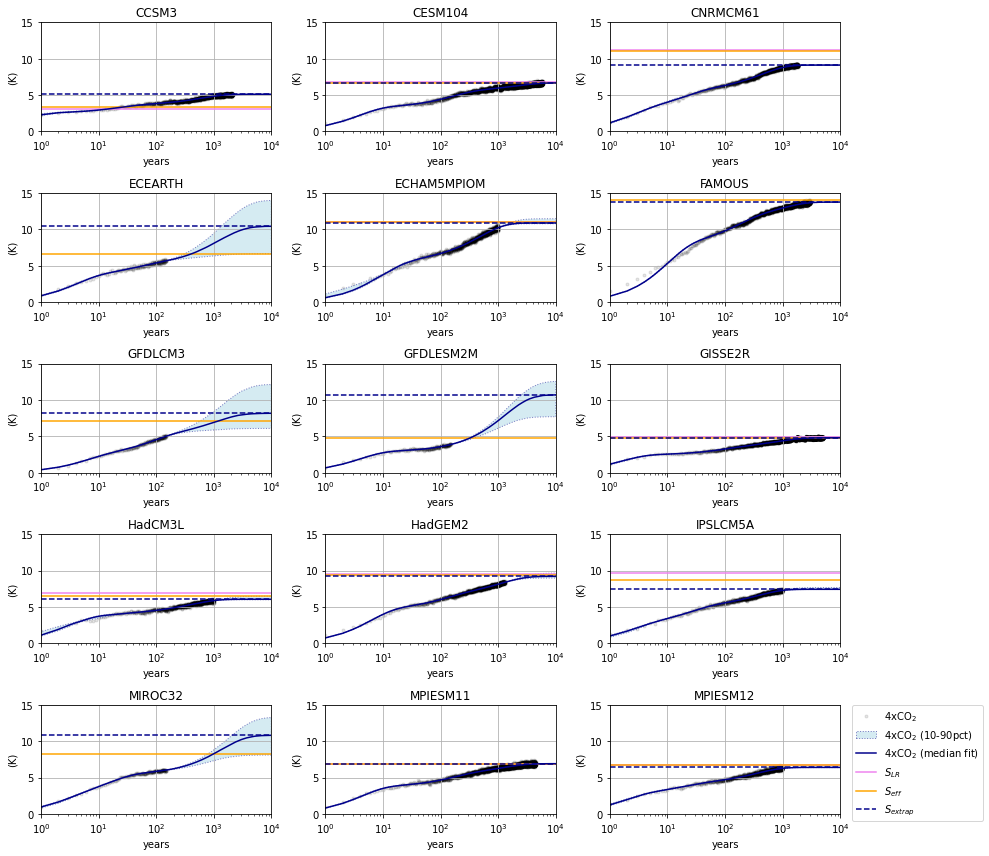
\includegraphics[width=\linewidth]{t_extrap_lrmip.png}
    \caption{Global mean temperature anomaly with respect to the last 500 available years of the PIControl simulation, plotted as a function of time (log scale) for the members of the LongrunMIP ensemble.  Black points show annual global mean TAS anomalies from the abrupt4xCO2 simulation.  Thick Blue lines show the median TOA timeseries using the ensemble of 3 timescale exponential models from the posterior fitted MCMC distribution (see Section \ref{sec_methods}).  Shaded regions and thin dotted lines show the 10th and 90th percentiles the fitted ensemble projections.  Dashed horizontal line illustrates $S_{extrap}$ (calculated using the 3 timescale model), yellow is $S_{eff}$ (effective climate sensitivity calculated using the first 150 years) and purple is $S_{LR}$ (effective climate sensitivity calculated using the last 15$\%$ of warming.}
    \label{fig:t_extrap_lrmip}
\end{figure}

We note that there is significant model diversity in the behaviour of models in the approach to equilibrium, and in the consistency of different approaches.  Some models  (CESM104, HadCM3L, FAMOUS, MPIESM11 and MPIESM12) behave as expected, showing near-zero equilibrium TOA balance in both PICTRL and in the extrapolated ABRUPT4X simulation.  In these simulations, $S_{LR}$ and $S_{extrap}$ are nearly identical.  

However, one model (CNRMCM61) has non-zero equilibrium TOA energetic balance, both in PICTRL and ABRUPT4X simulations, where there is a significant difference between the equilibrium energetic imbalance in PICTRL and ABRUPT4X (see Figure \ref{fig:extrap_lrmip}), which biases both $S_{LR}$ and $S_{eff}$.  CNRMCM61 exhibits relatively constant feedbacks on century and millennial timescales, so $S_{LR}$ and $S_{eff}$ are similar (5.62K, 5.52K respectively), but $S_{extrap}$, which is well fitted by the data is significantly lower (4.56$\pm$0.01K), see Figure \ref{fig:t_extrap_lrmip}) due to the differing estimated equilibrium energetic imbalance in ABRUPT4X and PICTRL simulations.  

A second model (HasCM3L) appears to show a control simulation in near energetic balance, but an ABRUPT4X simulation which converges to a state of energetic imbalance (Figure \ref{fig:extrap_lrmip}).  This, in turn introduces a source of potential bias in the estimate of effective climate sensitivity if the system is converging to a non-equilibrated state - implying that the control simulation may be tuned to exhibit energetic balance but the equilibrated 4xCO2 state is subject to an energy leak.  The fitted extrapolated sensitivity $S_{extrap}$ (3.03K, see Table \ref{tbl:LRMIP}) indicates a lower climate sensitivity than implied by $S_{LR}$ (3.49K) and $S_{eff}$ (3.29K).

Another model (CCSM3) appears to show an ABRUPT4X simulation which converges to energetic balance, but a PICTRL simulation which does not.  If TOA anomalies are measured relative to the last 500 years of the control simulation, $S_{LR}=1.52K$ and $S_{eff}=1.69K$, much lower than the published value of $S_{eff}=2.7K$ \citep{kiehl2006climate}.  If absolute TOA imbalances are used (rather than anomalies with respect to $R_{CTRL}$), $S_{LR}$ and $S_{eff}$  are consistent with \cite{kiehl2006climate}.  $S_{extrap}$ has a constrained value range of 2.56K ($\pm$ 0.01K) - again close to the published value in \cite{kiehl2006climate}.  Given this, we consider it possible that there is an irregularity in the reporting of TOA net flux in the PICTRL simulation from this model.

We find, in practise, that 1000 years of simulation are necessary to confidently fit the 3 mode model to the 4xCO2 simulation, such that the fitted equilibrium sensitivity is known to within 0.1K (see Table \ref{tbl:LRMIP}. A number of models have insufficient years in the LongrunMIP 4xCO2 simulation to be confident in the extrapolated temperature and energetic balance when fitting the 3 timescale model (ECEARTH, GFDLCM3, GFDLESM2M, MIROC32).  For these models, the exponential fitting approach can make no confident assessment of whether the ABRUPT4X simulation is converging to an equilibrated state.  One model (ECHAM5MPIOM) has insufficient data in both ABRUPT4X and PICONTROL simulations to be confident in equilibration tendencies using the timescale fitting approach (see Figure \ref{fig:extrap_lrmip}).

Looking at the wider CMIP5 and CMIP6 ensembles, it is apparent that a large number of models may be potentially subject to these biases, given that large flux imbalances are present in the control state \ref{fig:histo}.  However, the standard CMIP5 and CMIP6 simulations contain insufficient data to fully assess the extrapolated equilibrium climate sensitivity (or the extrapolated energetic imbalance in ABRUPT4X) using the 3 mode fitting approach (see Figure \ref{fig:histo}), though in most cases the uncertainties in the fitted solution generally allow for equilibrium values which are higher then the effective climate sensitivity as assessed over the first 150 years of simulation.  Only a small number of models allow for fitted solutions which have a lower ECS than the effective value (MIROC5, CNRMESM2.1, ACCESS-CM2).  One of these cases (CNRMCM6.1) is a close relative of the CNRMESM2.1 - the LongrunMIP simulation which we identified to be potentially subject to biases owing to energetic imbalances in the 4xCO2 equilibrium state.



\begin{figure}
    \centering
    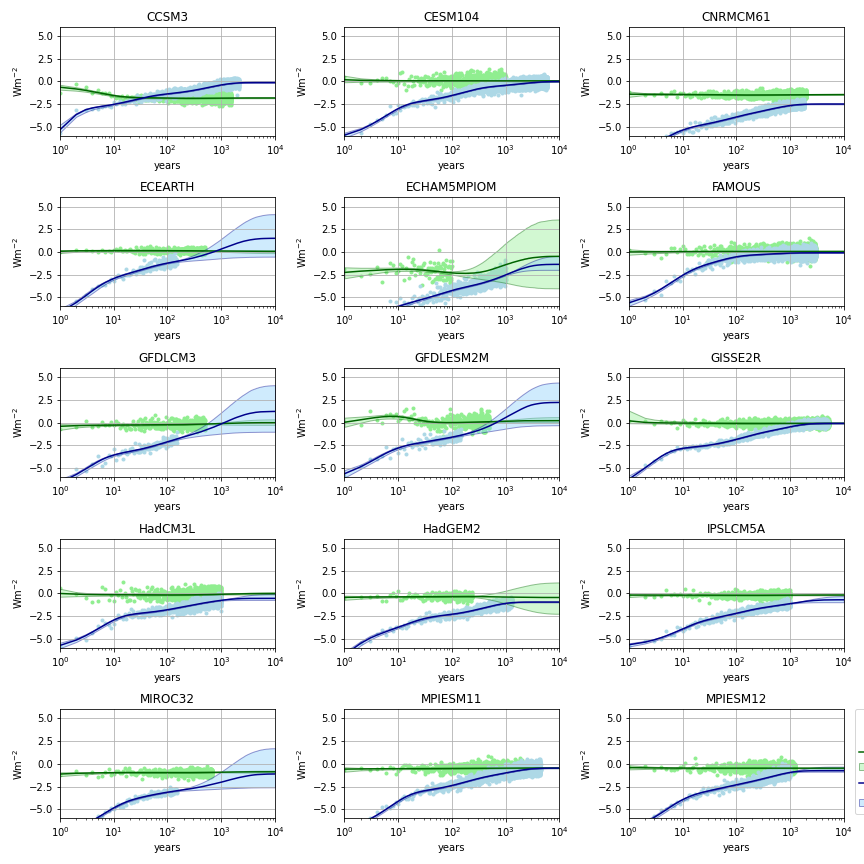
\includegraphics[width=\linewidth]{extrap_lrmip.png}
    \caption{Top of atmosphere net radiative imbalance plotted as a function of time (log scale) for the members of the LongrunMIP ensemble.  Blue and green points show annual mean upgoing net radiative flux from the Control integration and the abrupt4xCO2 simulation respectively.  Thick blue and green lines show the median TOA timeseries using the ensemble of 3 timescale exponential models from the posterior fitted MCMC distribution (see Section \ref{sec_methods}).  Shaded regions and thin lines show the 10th and 90th percentiles the fitted ensemble projections.}
    \label{fig:extrap_lrmip}
\end{figure}



\begin{figure}
    \centering
    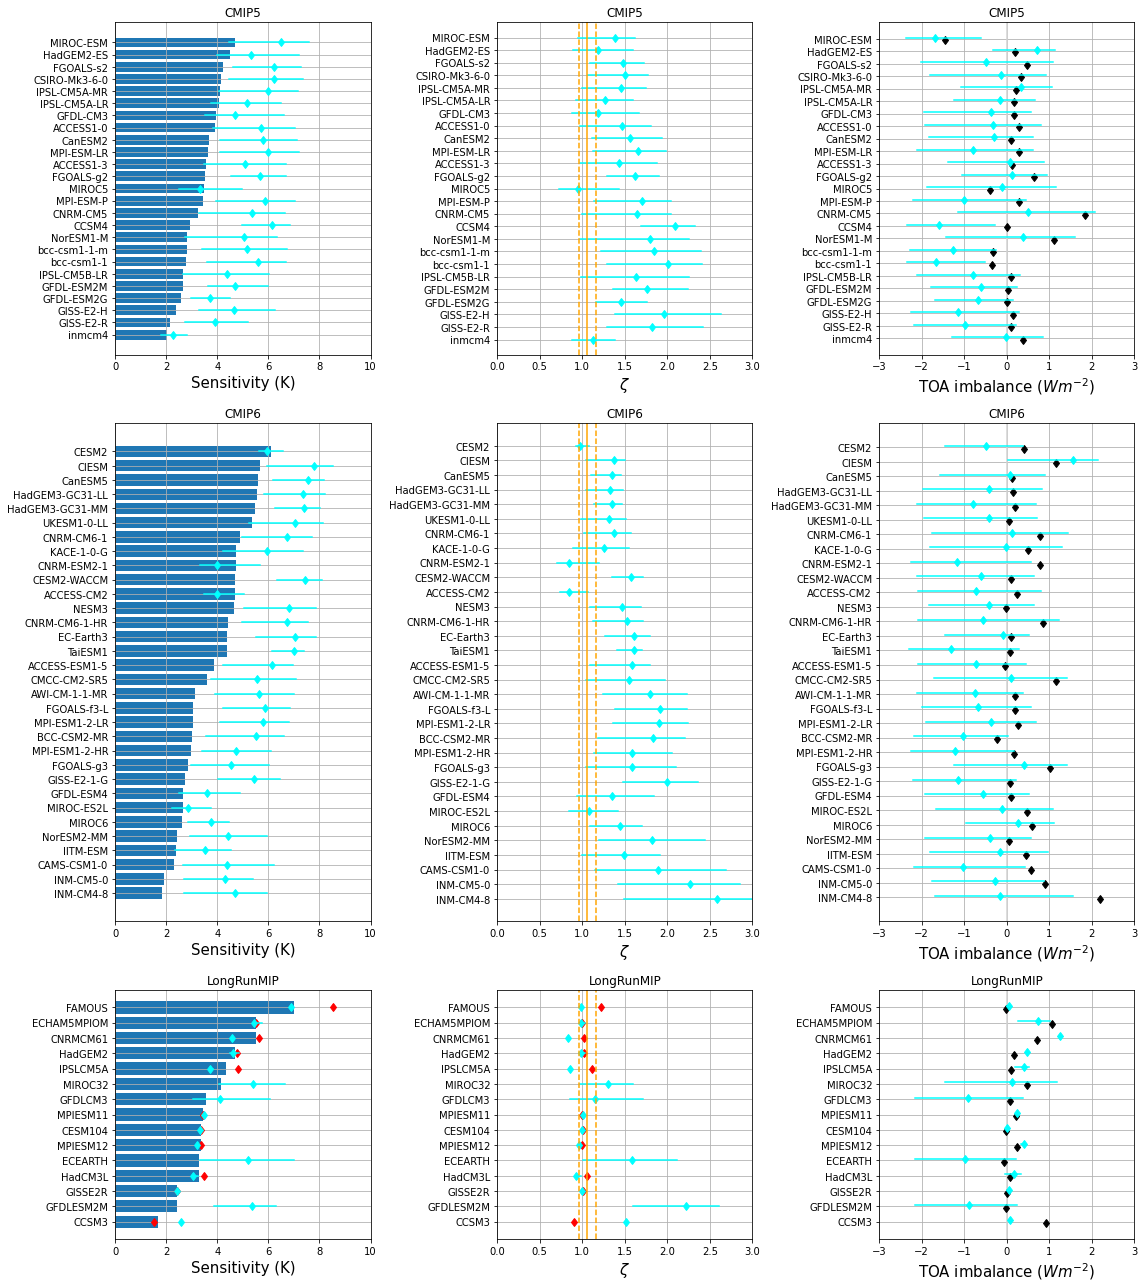
\includegraphics[width=\linewidth]{histo.png}
    \caption{Barplots summarising results for three model ensembles, CMIP5 (top row), CMIP6 (middle row) and LongRunMIP (bottom row).  Left hand column shows different measures of equilibrium climate sensitivity.  Solid blue bars show the effective climate sensitivity as measured from the first 150 years of the abrupt4xCO2 experiment, using temperature and net TOA anomalies from PICTRL values the last available 500 years.  Light blue diamond and whiskers show the median, 10th and 90th percentiles of the fitted distribution of equilibrium warming values for the 3 timescale model (fitted to all available years of the abrupt4xCO2 global mean temperature anomaly timeseries).  For simulations of 500 years or longer, an additional effective climate sensitivity is calculated (following \cite{rugenstein2020equilibrium}), using annual values for years corresponding to the last 15$\%$ of warming (as a fraction of the average annual mean temperature anomaly in the last 10 years of the timeseries), shown in red.  The central column shows the ratio of equilibrium climate sensitivity to effective climate sensitivity ($\zeta$ as defined in \cite{sherwood2020assessment}), for both the timescale fitting approach (cyan errorbars) and the effective sensitivity estimate using the the last 15$\%$ of warming (red diamonds). }
    \label{fig:histo}
\end{figure}



\conclusions  
We have considered here an alternative approach for calculating long term tendencies of temperature and planetary energetic imbalance from a simulation in which atmospheric carbon dioxide concentration is instantaneously perturbed.  This approach relies on the assumption that the evolution of the system can be represented as a sum of decaying exponential terms with differing timescales.  In order to produce confident results, the approach requires additional data beyond the conventional 150 years provided in CMIP climate simulation archives, however, an existing project, LongrunMIP, provides multi-millennial simulations which allow for a confident application of this approach.

We find that this approach highlights some potential limitations and biases associated with using effective climate sensitivity to predict equilibrium warming in response to CO2 perturbations. 
It has been observed before that energetic imbalances exist in some models in the CMIP archive \cite{rugenstein2019longrunmip}, and in this study we show that such control state radiative imbalances are relatively widespread in CMIP5 and CMIP6.  

The conventional assumption used to calculate effective climate sensitivity in these cases is that such imbalances remain constant, such that radiative anomalies from the control state can be used to calculate the effective climate sensitivity.  Critically, in some LongrunMIP simulations, we observe that energetic imbalances exist both in the control state, and in the extrapolated tendencies of the simulations with CO2 perturbations - but those imbalances are themselves state-dependent.  This undermines the concept of effective climate sensitivity - if we do not know what the radiative imbalance will be when temperatures stabilise in an abrupt4x simulation, we in turn cannot predict the climate sensitivity with any confidence.

In practise, only some models in CMIP5 and CMIP6 appear to exhibit radiative imbalances in the control state (see Figure \ref{fig:histo}. 


%% \conclusions[modified heading if necessary]


%% The following commands are for the statements about the availability of data sets and/or software code corresponding to the manuscript.
%% It is strongly recommended to make use of these sections in case data sets and/or software code have been part of your research the article is based on.

\codeavailability{TEXT} %% use this section when having only software code available


\dataavailability{TEXT} %% use this section when having only data sets available


\codedataavailability{TEXT} %% use this section when having data sets and software code available


\sampleavailability{TEXT} %% use this section when having geoscientific samples available


\videosupplement{TEXT} %% use this section when having video supplements available


\appendix
\section{}    %% Appendix A

\subsection{}     %% Appendix A1, A2, etc.


\noappendix       %% use this to mark the end of the appendix section. Otherwise the figures might be numbered incorrectly (e.g. 10 instead of 1).

%% Regarding figures and tables in appendices, the following two options are possible depending on your general handling of figures and tables in the manuscript environment:

%% Option 1: If you sorted all figures and tables into the sections of the text, please also sort the appendix figures and appendix tables into the respective appendix sections.
%% They will be correctly named automatically.

%% Option 2: If you put all figures after the reference list, please insert appendix tables and figures after the normal tables and figures.
%% To rename them correctly to A1, A2, etc., please add the following commands in front of them:

\appendixfigures  %% needs to be added in front of appendix figures


\appendixtables   %% needs to be added in front of appendix tables

%% Please add \clearpage between each table and/or figure. Further guidelines on figures and tables can be found below.


\begin{table*}[t]
\small
\begin{tabular}{llrrlrllr}
\toprule
       Model & Years &  $S_{eff}$ &  $S_{LR}$ &       $S_{extrap}$ & $\zeta_{LG}$ &   $\zeta_{extrap}$ &    $R^{4x}_{extrap}$ & $R^{CTRL}_0$ \\
\midrule
       CCSM3 &  2120 &       1.69 &      1.52 &  2.56 (2.55,2.56) &    0.90 &  1.51 (1.51,1.51) &    0.06 (0.05,0.08) &         0.92 \\
     CESM104 &  5900 &       3.36 &      3.38 &  3.34 (3.34,3.34) &    1.01 &    1.0 (0.99,1.0) &    0.01 (-0.0,0.02) &        -0.03 \\
    CNRMCM61 &  1850 &       5.52 &      5.62 &  4.56 (4.56,4.57) &    1.02 &  0.83 (0.83,0.83) &    1.26 (1.25,1.27) &         0.72 \\
     ECEARTH &   150 &       3.30 &         - &  5.22 (3.33,6.99) &       - &  1.58 (1.01,2.12) &  -0.98 (-2.15,0.21) &        -0.06 \\
 ECHAM5MPIOM &  1001 &       5.53 &      5.52 &  5.44 (5.39,5.73) &    1.00 &  0.98 (0.97,1.04) &    0.74 (0.25,1.01) &         1.06 \\
      FAMOUS &  3000 &       7.01 &      8.55 &  6.88 (6.86,6.89) &    1.22 &  0.98 (0.98,0.98) &    0.04 (0.01,0.05) &        -0.03 \\
     GFDLCM3 &   150 &       3.55 &         - &  4.09 (3.05,6.07) &       - &  1.15 (0.86,1.71) &   -0.9 (-2.17,0.38) &         0.09 \\
   GFDLESM2M &   150 &       2.41 &         - &  5.35 (3.85,6.28) &       - &   2.22 (1.6,2.61) &  -0.89 (-2.15,0.24) &        -0.02 \\
     GISSE2R &  5001 &       2.42 &      2.44 &     2.4 (2.4,2.4) &    1.01 &   0.99 (0.99,1.0) &    0.04 (0.04,0.05) &         0.01 \\
     HadCM3L &  1000 &       3.29 &      3.49 &   3.03 (3.0,3.24) &    1.06 &  0.92 (0.91,0.99) &   0.18 (-0.05,0.34) &         0.07 \\
     HadGEM2 &  1299 &       4.70 &      4.78 &  4.61 (4.49,4.83) &    1.02 &  0.98 (0.96,1.03) &     0.48 (0.45,0.5) &         0.18 \\
    IPSLCM5A &  1000 &       4.35 &      4.82 &   3.72 (3.7,3.84) &    1.11 &  0.86 (0.85,0.88) &     0.41 (0.2,0.52) &         0.09 \\
     MIROC32 &   150 &       4.15 &         - &  5.41 (4.06,6.64) &       - &   1.31 (0.98,1.6) &   0.13 (-1.45,1.18) &         0.46 \\
    MPIESM11 &  4459 &       3.45 &      3.44 &  3.46 (3.46,3.47) &    1.00 &    1.0 (1.0,1.01) &    0.24 (0.23,0.28) &         0.22 \\
    MPIESM12 &  1000 &       3.35 &      3.34 &  3.21 (3.19,3.22) &    1.00 &  0.96 (0.95,0.96) &     0.4 (0.34,0.44) &         0.24 \\
\bottomrule
\end{tabular}
\label{tbl:LRMIP}

\end{table*}
\clearpage
\begin{table*}[t]
\small
\begin{tabular}{llrrlrllr}
\toprule
       Model & Years &  $S_{eff}$ &  $S_{LR}$ &       $S_{extrap}$ & $\zeta_{LG}$ &   $\zeta_{extrap}$ &    $R^{4x}_{extrap}$ & $R^{CTRL}_0$ \\
\midrule
     ACCESS1-0 &   150 &       3.90 &         - &  5.73 (3.82,7.05) &       - &  1.47 (0.98,1.81) &   -0.33 (-1.93,0.81) &         0.29 \\
     ACCESS1-3 &   151 &       3.56 &         - &  5.09 (3.47,6.68) &       - &  1.43 (0.98,1.88) &    0.07 (-1.37,0.87) &         0.11 \\
         CCSM4 &   151 &       2.94 &         - &  6.14 (4.99,6.84) &       - &  2.09 (1.69,2.32) &  -1.59 (-2.34,-0.28) &        -0.00 \\
      CNRM-CM5 &   150 &       3.26 &         - &  5.36 (3.27,6.66) &       - &   1.64 (1.0,2.05) &     0.5 (-1.15,2.07) &         1.84 \\
 CSIRO-Mk3-6-0 &   150 &       4.14 &         - &  6.22 (4.44,7.34) &       - &   1.5 (1.07,1.77) &   -0.13 (-1.81,0.92) &         0.33 \\
       CanESM2 &   150 &       3.69 &         - &  5.78 (4.09,7.13) &       - &  1.57 (1.11,1.93) &   -0.29 (-1.83,0.62) &         0.10 \\
     FGOALS-g2 &   258 &       3.52 &         - &   5.69 (4.55,6.7) &       - &   1.61 (1.29,1.9) &    0.12 (-1.05,0.94) &         0.63 \\
     FGOALS-s2 &   150 &       4.22 &         - &  6.23 (4.61,7.29) &       - &  1.48 (1.09,1.73) &   -0.48 (-2.03,1.08) &         0.48 \\
      GFDL-CM3 &   150 &       3.96 &         - &   4.68 (3.5,6.62) &       - &  1.18 (0.88,1.67) &   -0.36 (-1.95,0.58) &         0.16 \\
    GFDL-ESM2G &   300 &       2.56 &         - &  3.73 (2.97,4.51) &       - &  1.45 (1.16,1.76) &    -0.68 (-1.7,0.14) &        -0.00 \\
    GFDL-ESM2M &   300 &       2.67 &         - &  4.71 (3.64,5.99) &       - &  1.76 (1.36,2.24) &    -0.6 (-1.79,0.24) &         0.03 \\
     GISS-E2-H &   151 &       2.38 &         - &  4.66 (3.29,6.24) &       - &  1.96 (1.38,2.63) &   -1.15 (-2.25,0.29) &         0.14 \\
     GISS-E2-R &   151 &       2.14 &         - &  3.89 (2.75,5.19) &       - &  1.82 (1.29,2.42) &   -0.99 (-2.18,0.21) &         0.10 \\
    HadGEM2-ES &   152 &       4.49 &         - &  5.33 (3.98,7.18) &       - &   1.19 (0.89,1.6) &     0.7 (-0.33,1.14) &         0.20 \\
  IPSL-CM5A-LR &   260 &       4.06 &         - &  5.15 (3.74,6.49) &       - &   1.27 (0.92,1.6) &   -0.16 (-1.25,0.67) &         0.17 \\
  IPSL-CM5A-MR &   140 &       4.10 &         - &  5.99 (4.08,7.15) &       - &   1.46 (1.0,1.74) &    0.33 (-1.08,1.06) &         0.22 \\
  IPSL-CM5B-LR &   160 &       2.67 &         - &  4.36 (2.64,6.02) &       - &  1.63 (0.99,2.25) &   -0.79 (-2.12,0.32) &         0.09 \\
     MIROC-ESM &   150 &       4.69 &         - &  6.48 (4.44,7.58) &       - &  1.38 (0.95,1.62) &  -1.68 (-2.37,-0.61) &        -1.44 \\
        MIROC5 &   151 &       3.46 &         - &    3.3 (2.5,4.96) &       - &  0.95 (0.72,1.43) &    -0.1 (-1.87,1.17) &        -0.39 \\
    MPI-ESM-LR &   150 &       3.63 &         - &   6.0 (4.09,7.18) &       - &  1.66 (1.13,1.98) &      -0.8 (-2.1,0.6) &         0.28 \\
     MPI-ESM-P &   150 &       3.45 &         - &  5.85 (3.93,7.05) &       - &   1.7 (1.14,2.05) &   -0.99 (-2.21,0.46) &         0.28 \\
     NorESM1-M &   150 &       2.81 &         - &  5.03 (2.72,6.34) &       - &  1.79 (0.97,2.26) &    0.39 (-1.42,1.61) &         1.11 \\
    bcc-csm1-1 &   150 &       2.79 &         - &   5.59 (3.6,6.71) &       - &    2.0 (1.29,2.4) &  -1.66 (-2.34,-0.51) &        -0.35 \\
  bcc-csm1-1-m &   150 &       2.80 &         - &  5.17 (3.41,6.71) &       - &  1.84 (1.22,2.39) &  -1.27 (-2.28,-0.26) &        -0.32 \\
        inmcm4 &   150 &       2.03 &         - &  2.28 (1.78,2.81) &       - &  1.12 (0.88,1.38) &   -0.02 (-1.28,0.84) &         0.38 \\
\bottomrule
\end{tabular}
\label{tbl:CMIP5}

\end{table*}

\clearpage

\begin{table*}[t]
\small
\begin{tabular}{llrrlrllr}
\toprule
       Model & Years &  $S_{eff}$ &  $S_{LR}$ &       $S_{extrap}$ & $\zeta_{LG}$ &   $\zeta_{extrap}$ &    $R^{4x}_{extrap}$ & $R^{CTRL}_0$ \\
\midrule
      ACCESS-CM2 &   150 &       4.71 &         - &  3.97 (3.47,5.03) &       - &  0.84 (0.74,1.07) &   -0.72 (-2.09,0.8) &         0.25 \\
   ACCESS-ESM1-5 &   150 &       3.87 &         - &  6.13 (4.21,6.95) &       - &   1.59 (1.09,1.8) &  -0.73 (-2.09,0.45) &        -0.04 \\
   AWI-CM-1-1-MR &   151 &       3.14 &         - &  5.64 (3.91,6.99) &       - &   1.8 (1.24,2.23) &  -0.75 (-2.12,0.39) &         0.20 \\
     BCC-CSM2-MR &   151 &       3.00 &         - &  5.51 (3.54,6.62) &       - &  1.83 (1.18,2.21) &  -1.03 (-2.18,0.03) &        -0.24 \\
     CAMS-CSM1-0 &   150 &       2.31 &         - &  4.37 (2.67,6.23) &       - &  1.89 (1.15,2.69) &  -1.04 (-2.19,0.43) &         0.56 \\
           CESM2 &   400 &       6.11 &         - &  5.96 (5.64,6.56) &       - &  0.98 (0.92,1.07) &  -0.49 (-1.44,0.37) &         0.40 \\
     CESM2-WACCM &   150 &       4.71 &         - &   7.43 (6.33,8.1) &       - &  1.58 (1.34,1.72) &   -0.62 (-2.1,0.64) &         0.10 \\
           CIESM &   150 &       5.69 &         - &   7.8 (5.95,8.51) &       - &   1.37 (1.05,1.5) &    1.55 (0.03,2.14) &         1.17 \\
    CMCC-CM2-SR5 &   165 &       3.59 &         - &  5.57 (3.75,7.08) &       - &  1.55 (1.04,1.97) &    0.1 (-1.72,1.41) &         1.15 \\
      CNRM-CM6-1 &   150 &       4.90 &         - &  6.73 (4.98,7.73) &       - &  1.37 (1.02,1.58) &   0.11 (-1.76,1.44) &         0.78 \\
   CNRM-CM6-1-HR &   150 &       4.41 &         - &  6.74 (4.98,7.54) &       - &  1.53 (1.13,1.71) &  -0.56 (-2.09,1.22) &         0.86 \\
     CNRM-ESM2-1 &   150 &       4.73 &         - &   4.0 (3.33,5.68) &       - &    0.84 (0.7,1.2) &  -1.16 (-2.25,0.56) &         0.78 \\
         CanESM5 &   151 &       5.59 &         - &  7.54 (6.18,8.16) &       - &   1.35 (1.1,1.46) &    0.07 (-1.56,0.9) &         0.12 \\
       EC-Earth3 &   160 &       4.37 &         - &  7.03 (5.53,7.86) &       - &   1.61 (1.27,1.8) &  -0.09 (-1.45,0.52) &         0.10 \\
     FGOALS-f3-L &   160 &       3.07 &         - &  5.87 (4.24,6.84) &       - &  1.91 (1.38,2.23) &  -0.67 (-1.98,0.56) &         0.19 \\
       FGOALS-g3 &   152 &       2.86 &         - &  4.53 (2.97,6.01) &       - &   1.59 (1.04,2.1) &    0.4 (-1.24,1.42) &         1.01 \\
       GFDL-ESM4 &   150 &       2.67 &         - &   3.61 (2.51,4.9) &       - &  1.35 (0.94,1.84) &  -0.55 (-1.92,0.53) &         0.10 \\
     GISS-E2-1-G &   151 &       2.73 &         - &  5.45 (4.04,6.46) &       - &   2.0 (1.48,2.37) &  -1.15 (-2.21,0.22) &         0.08 \\
 HadGEM3-GC31-LL &   150 &       5.57 &         - &   7.37 (5.84,8.2) &       - &  1.32 (1.05,1.47) &  -0.42 (-1.97,0.84) &         0.14 \\
 HadGEM3-GC31-MM &   150 &       5.48 &         - &  7.41 (6.25,8.02) &       - &  1.35 (1.14,1.46) &    -0.79 (-2.1,0.7) &         0.19 \\
        IITM-ESM &   165 &       2.37 &         - &  3.52 (2.35,4.54) &       - &  1.48 (0.99,1.91) &  -0.15 (-1.81,0.96) &         0.45 \\
       INM-CM4-8 &   150 &       1.82 &         - &  4.68 (2.71,5.96) &       - &  2.58 (1.49,3.28) &  -0.15 (-1.69,1.55) &         2.19 \\
       INM-CM5-0 &   150 &       1.90 &         - &  4.29 (2.69,5.41) &       - &  2.26 (1.42,2.85) &  -0.27 (-1.77,0.87) &         0.90 \\
      KACE-1-0-G &   151 &       4.74 &         - &  5.94 (4.23,7.35) &       - &  1.25 (0.89,1.55) &   -0.03 (-1.81,1.3) &         0.49 \\
      MIROC-ES2L &   150 &       2.66 &         - &  2.87 (2.24,3.77) &       - &  1.08 (0.84,1.42) &   -0.1 (-1.67,1.09) &         0.48 \\
          MIROC6 &   250 &       2.62 &         - &  3.77 (2.87,4.47) &       - &  1.44 (1.09,1.71) &    0.25 (-0.96,1.1) &         0.60 \\
   MPI-ESM1-2-HR &   165 &       2.97 &         - &  4.71 (3.39,6.11) &       - &  1.59 (1.14,2.06) &  -1.22 (-2.25,0.16) &         0.17 \\
   MPI-ESM1-2-LR &   165 &       3.03 &         - &  5.78 (4.12,6.82) &       - &   1.9 (1.36,2.25) &   -0.38 (-1.9,0.69) &         0.26 \\
           NESM3 &   150 &       4.64 &         - &  6.83 (5.06,7.85) &       - &  1.47 (1.09,1.69) &  -0.42 (-1.83,0.64) &        -0.02 \\
      NorESM2-MM &   150 &       2.44 &         - &  4.42 (2.91,5.95) &       - &   1.81 (1.2,2.44) &   -0.4 (-1.92,0.56) &         0.04 \\
         TaiESM1 &   150 &       4.36 &         - &  7.02 (6.14,7.41) &       - &   1.61 (1.41,1.7) &   -1.31 (-2.29,0.3) &         0.08 \\
     UKESM1-0-LL &   150 &       5.36 &         - &  7.04 (5.26,8.13) &       - &  1.31 (0.98,1.52) &  -0.42 (-1.94,0.71) &         0.05 \\
\bottomrule
\end{tabular}
\label{tbl:CMIP6}

\end{table*}

\authorcontribution{TEXT} %% this section is mandatory

\competinginterests{TEXT} %% this section is mandatory even if you declare that no competing interests are present

\disclaimer{TEXT} %% optional section

\begin{acknowledgements}
TEXT
\end{acknowledgements}




\bibliographystyle{copernicus}
\bibliography{sample_full.bib}


\end{document}
